\documentclass{article}


\usepackage[final]{nips_anon}


\usepackage[utf8]{inputenc} % allow utf-8 input
\usepackage[T1]{fontenc}    % use 8-bit T1 fonts
\usepackage{hyperref}       % hyperlinks
\usepackage{url}            % simple URL typesetting
\usepackage{booktabs}       % professional-quality tables
\usepackage{amsfonts}       % blackboard math symbols
\usepackage{nicefrac}       % compact symbols for 1/2, etc.
\usepackage{microtype}      % microtypography

% additional packages
\usepackage{graphicx} % more modern 
\usepackage{caption}
\usepackage{subcaption}
\usepackage{tikz}
\usepackage{dsfont}
\usepackage{amsmath}
\usepackage{amssymb}
\usepackage{amsthm}
\usepackage{times}
\usepackage{natbib}
\usepackage{algorithm}
\usepackage[noend]{algorithmic}
\usepackage{wrapfig}
%

\newif\ifsup\suptrue

\graphicspath{ {figures/} }
\usetikzlibrary{arrows,positioning,backgrounds} 
\tikzset{
    %Define standard arrow tip
    >=stealth',
    %Define style for boxes
    observed/.style={
           circle,
           rounded corners,
           draw=black, thick,
           minimum width=2.2em,
           minimum height=2.2em,
           font=\tiny,
           text centered,
           scale=.8,
           fill=blue!20!white},
     latent/.style={
           circle,
           rounded corners,
           draw=black, thick, dashed,
           minimum width=.5em,
           minimum height=.5em,
           font=\footnotesize,
           text centered,
           fill=black!10!white
           },
     empty/.style={
           circle,
           rounded corners,
           minimum width=.5em,
           minimum height=.5em,
           font=\footnotesize,
           text centered,
           },
    % Define arrow style
    pil/.style={
           o->,
           thick,
           shorten <=2pt,
           shorten >=2pt,},
    sh/.style={ shade, shading=axis, left color=red, right color=green,
    shading angle=45 }  
}

\newcommand{\defined}{\vcentcolon =}
\newcommand{\rdefined}{=\vcentcolon}
\newcommand{\E}[1]{\mathbb E\left[#1\right]}
\newcommand{\R}{\mathbb R}
\newcommand{\Var}{\operatorname{Var}}
\newcommand{\calF}{\mathcal F}
\newcommand{\sr}[1]{\stackrel{#1}}
\newcommand{\set}[1]{\left\{#1\right\}}
\newcommand{\ind}[1]{\mathds{1}\!\!\set{#1}}
\newcommand{\argmax}{\operatornamewithlimits{arg\,max}}
\newcommand{\argmin}{\operatornamewithlimits{arg\,min}}
\newcommand{\floor}[1]{\left \lfloor {#1} \right\rfloor}
\newcommand{\ceil}[1]{\left \lceil {#1} \right\rceil}
\newcommand{\eqn}[1]{\begin{align}#1\end{align}}
\newcommand{\eq}[1]{\begin{align*}#1\end{align*}}
\newcommand{\Ber}{\operatorname{Bernoulli}}
\renewcommand{\P}[1]{\operatorname{P}\left\{#1\right\}}
\newcommand{\Pri}[1]{\operatorname{P}_i\left\{#1\right\}}
\newcommand{\Prz}[1]{\operatorname{P}_0\left\{#1\right\}}
\newcommand{\bigo}[1]{\mathcal{O}\left( #1 \right)}
\newcommand{\bigotilde}[1]{\tilde{\mathcal{O}}\left( #1 \right)}
\newcommand{\bigtheta}[1]{\Theta\left( #1 \right)}
\newcommand{\bigthetatilde}[1]{\tilde{\Theta}\left( #1 \right)}
\newcommand{\bigomega}[1]{\Omega\left( #1 \right)}
\newcommand{\KL}{\operatorname{KL}}
\newcommand{\simpleregret}{R_T}
\newcommand{\Pij}[1]{\operatorname{P}_{ij}\!\left\{#1\right\}}
\newcommand{\Pkl}[1]{\operatorname{P}_{kl}\!\left\{#1\right\}}
\newcommand{\Q}[1]{\operatorname{Q}\left\{#1\right\}}
\newcommand{\EE}{\mathbb E}
\newcommand{\EEa}{\EE_a}
\newcommand{\Pns}[2]{\operatorname{P}_{#1}\left\{#2\right\}}
\newcommand{\Pn}[2]{\operatorname{P}\left\{#2|#1\right\}}
\newcommand{\parents}[1]{\operatorname{\mathcal{P}a}_{#1}}
\newcommand{\actions}{\mathcal{A}}
\newcommand{\calA}{\mathcal A}
\newcommand{\etc}{\textit{etc}}
\newcommand{\ie}{\textit{i.e.}}
\newcommand{\eg}{\textit{e.g.}}
\newcommand{\calP}{\mathcal P}
\newcommand{\x}{\boldsymbol{x}}
\newcommand{\Ps}{\operatorname{P}}

\theoremstyle{plain}
\newtheorem{theorem}{Theorem}
\newtheorem{proposition}[theorem]{Proposition}
\newtheorem{lemma}[theorem]{Lemma}
\newtheorem{corollary}[theorem]{Corollary}
\theoremstyle{definition}
\newtheorem{definition}[theorem]{Definition}
\newtheorem{assumption}[theorem]{Assumption}
\newtheorem{remark}[theorem]{Remark}
\newtheorem{example}[theorem]{Example}
\let\temp\epsilon
\let\epsilon\varepsilon

\title{Causal Bandits: Learning Good Interventions via Causal Inference}

% The \author macro works with any number of authors. There are two
% commands used to separate the names and addresses of multiple
% authors: \And and \AND.
%
% Using \And between authors leaves it to LaTeX to determine where to
% break the lines. Using \AND forces a line break at that point. So,
% if LaTeX puts 3 of 4 authors names on the first line, and the last
% on the second line, try using \AND instead of \And before the third
% author name.
\author{
  Finnian Lattimore \\
  Australian National University and Data61/NICTA \\
  \texttt{finn.lattimore@gmail.com} \\
   \And
   Tor Lattimore \\
   University of Alberta \\
   \texttt{tor.lattimore@gmail.com} \\
   \And
   Mark D. Reid \\
   Australian National University and Data61/NICTA \\
   \texttt{mark.reid@anu.edu.au} \\
}


\begin{document}
% \nipsfinalcopy is no longer used


\maketitle

\begin{abstract} 
We study the problem of using causal models to improve the rate at which good interventions can be learned online in a stochastic environment. 
Our formalism combines multi-arm bandits and causal inference to model a novel type of bandit feedback that is not exploited by existing approaches.
We propose a new algorithm that exploits the causal feedback and prove a bound on its simple regret that is strictly better (in all quantities) 
than algorithms that do not use the additional causal information.
\end{abstract} 
%\begin{tikzpicture}[background rectangle/.style={fill=olive!45}, show background rectangle]




%%%%%%%%%%%%%%%%%%%%%%%%%%%%%%%%%%%%%%%%%%%%%%%%%
% INTRODUCTION
%%%%%%%%%%%%%%%%%%%%%%%%%%%%%%%%%%%%%%%%%%%%%%%%%

\section{Introduction}
\label{sec:intro}
Medical drug testing, policy setting, and other scientific processes are commonly framed and analysed in the language of sequential experimental design and, in special cases, as bandit problems~\citep{Robbins1952,Chernoff1959}. 
In this framework, single actions (\eg, experiments or interventions) from a pre-determined set are repeatedly performed in 
order to evaluate their effectiveness via feedback from a single, real-valued reward signal.
We propose a generalisation of the standard model by assuming that, in additional to the reward signal, the learner observes the values of a number of covariates 
drawn from a probabilistic causal model~\citep{Pearl2000}.
Causal models are commonly used in disciplines where explicit experimentation may be difficult such as social science, demography and economics.
For example, when predicting the effect of changes to childcare subsidies on workforce participation, or school choice on grades. 
Results from causal inference relate observational distributions to interventional ones, allowing the outcome of an intervention to be predicted without
explicitly performing it.
By exploiting the causal information we show, theoretically and empirically, how non-interventional observations can be used to improve the rate at 
which high-reward actions can be identified.

The type of problem we are concerned with is best illustrated with an example. 
Consider a farmer wishing to optimise the yield of her crop. 
She knows that crop yield is only affected by temperature, a particular soil nutrient, and moisture level but the precise effect of their combination is unknown.
In each season the farmer has enough time and money to intervene and control at most one of these variables:
deploying shade or heat lamps will set the temperature to be low or high; the nutrient can be added or removed a through a choice of fertilizer; and irrigation or rain-proof covers will keep the soil wet or dry.
When not intervened upon, the temperature, soil, and moisture vary naturally from season to season due to weather conditions and these are all observed along with the final crop yield at the end of each season.
How might the farmer best experiment to identify the single, highest yielding intervention in a limited number of seasons?
%without sacrificing too much crop yield (relative to always choosing the best intervention) in the process?


\subsection{Contributions}

This paper takes the first step towards formalising and solving problems such as the one above. 
In \S\ref{sec:defs} we formally introduce \emph{causal bandit problems} in which interventions are treated as arms in a bandit problem but their influence on the reward --- along with any other observations --- is assumed to conform to a known causal graph. 
We show that our causal bandit framework subsumes the classical bandits (no additional observations) and contextual stochastic bandit problems (observations are revealed before an intervention is chosen) before focusing on the case where, like the above example, observations occur \emph{after} each intervention is made.

We focus on the simple regret, which measures the difference between the return of the optimal action and that of the action chosen by the algorithm after $T$ rounds.
In \S\ref{sec:simple-regret} we analyse a specific family of causal bandit problems that we call \emph{parallel bandit} problems in which $N$ factors affect the reward independently and there are $2N$ possible interventions.
We propose a simple causal best arm identification algorithm (Algorithm~\ref{alg:simple}) for this problem and show that up to logarithmic factors it enjoys minimax optimal
simple regret guarantees of $\tilde\Theta(\sqrt{m/T})$ where $m$ depends on the causal model and may be much smaller than $N$.
In contrast, existing best arm identification algorithms suffer $\Omega(\sqrt{N/T})$ simple regret.
This shows theoretically the value of our framework over the traditional bandit problem. 
Experiments in \S\ref{sec:experiments} further demonstrate the value of causal models in this framework.
\todom{Mention cumulative regret?}

In the general casual model interventions and observations may have a complex relationship. 
In \S\ref{sec:simple-regret-general} we propose an novel algorithm inspired by importance-sampling that a) enjoys sub-linear regret equivalent to the optimal rate in the parallel bandit setting and b) captures many of the intricacies of sharing information in a causal graph in the general case. 
As in the parallel bandit case, the regret guarantee is often significantly better than $O(\sqrt{N/T})$ and never worse, where $N$ is the number of available interventions.



\subsection{Related Work}

As alluded to above, causal bandit problems with $N$ possible interventions can be treated as a classical $N$-armed bandit problem by simply ignoring the causal model and extra observations that are revealed each round.
In the farming example, the farmer could treat the six possible interventions are arms, ignore the observations of the non-intervened variables, and apply an algorithm such as UCB~\cite{Auer1995} with well understood regret guarantees.
However, as we show in \S\ref{sec:simple-regret}, this approach ignores the extra information available in the non-intervened variables and subsequently yields sub-optimal performance.

Bandit problems with side information are commonly referred to as ``contextual bandits'' and have been well studied in recent years~\cite{Langford2008,Agarwal2014}.
Our framework bears a superficial similarity to contextual bandit problems since the extra observations on non-intervened variables might be viewed as context for selecting an intervention. 
However, a crucial difference is that in our model the extra observations are only revealed \emph{after} selecting an intervention and cannot be used as context.
We discuss the relationship between causal and contextual bandits further in \S\ref{sec:defs} and leave their combination as future work.

There has been a significant amount of recent work which proposes alternative modes of feedback within the bandit setting \citep{Alon2015} which, at first glance, may appear applicable. Indeed, we show in \S~\ref{sec:discussion}, that it is possible to applying these existing results to our problem, however the resulting regret is $\bigo{\sqrt{NT}}$, again with a sub-optimal dependence on $N$.

\todom{Rework rest of intro}

%Problems requiring choosing an action under uncertainty are rife in all areas of human endeavour. For many problems, actions may be chosen sequentially, allowing the agent to learn from the outcome of early choices to improve later ones. 

% A widely used framework for sequential decision making is the multi-armed bandit. In the classic multi-armed bandit setting there is a finite set of available actions, each associated with a distribution over rewards which is unknown but stationary. At each timestep the agent selects an action and receives a reward sampled i.i.d from the corresponding reward distribution. The performance of bandit algorithms is described by the regret: the difference in the expected reward obtained by the algorithm and the reward that could be obtained if the optimal action was selected at every timestep. 


% We take a first step towards unifying these approaches by considering a variant of the stochastic multi-armed bandit problem where we have prior knowledge of the causal structure governing the available actions. 

% A natural way to connect the causal framework with the bandit setting is to model the problem as a causal directed acyclic graph. Each possible assignment of variables to values is an action (bandit arm). The reward could be a general function of the action selected and the final state of the graph. However for simplicity, we will consider the reward to be the value of a single specified node minus the cost of the selected action. The number of actions grows exponentially with the number of variables in the graph, making it important to use algorithms that take account of the graph structure to reduce the search space. 

% Problems framed in this way take on characteristics of different bandit settings depending on the assumptions we make about what subset of actions can be taken, what variables are observable and whether they are observed before or after an action is selected. If feedback is received only on the reward node then the do-calculus can be applied to eliminate some actions immediately, before any experiments are performed and then a standard bandit algorithm can be run on the remaining actions. 

% If we receive feedback on additional nodes the problem can be more interesting. In addition to being able to eliminate some actions prior to sampling any data as in the previous case, taking one action may give us some information on actions that were not selected. 

% We consider a bandit problem where the actions and reward are represented by a specific causal graph that demonstrates this interesting structure. We develop an algorithm to leverage the information provided by this structure and demonstrate it substantially outperforms standard bandit algorithms applied to the same problem where the number of actions is large.

There has been substantial recent work into extending bandit algorithms to incorporate additional assumptions and deal with more complex feedback structures. Algorithms with strong guarantees have been developed for linear bandits [], generalized linear bandits, gaussian process bandits [], etc. There is also an active line of research into bandits with feedback defined by a graph. Actions are modelled as nodes in the graph and the agent observes rewards for each action connected to the selected action []. The novelty of our work is that we assume prior knowledge of the causal structure but not the functional form of the relationship between variables.   

% Partial monitoring is a very general framework for for decoupling the feedback from the action and reward. It can be used to classify problems into one of four categories, trivial with no regret, easy with $R_T = \bigthetatilde{\sqrt{T}}$ , hard with $R_T = \bigtheta{T^{2/3}}$ and hopeless with $R_T = \bigomega{T}$ \cite{Bartok2014}. Partial monitoring algorithms yield results that are optimal with respect the horizon $T$ but not other parameters, such as $K$, which is the key focus of incorporating causal structure. 

Two pieces of recent work also consider using causal models in bandit problems.
Although \citet{Bareinboim2015} also use causal inference to improve the chance of choosing an optimal arm, their work differs from our in two key ways. Firstly, their focus is on correcting the effects of unobserved confounding variables whereas we assume all variables are observable. Secondly, they do not assume their learning algorithm has access to a causal graph and instead use a form of contextual randomization to improve reward estimates in a Thompson sampling-style algorithm. \citet{Ortega2014thompson} also present an analysis and extension of Thompson sampling assuming actions are causal interventions. Their focus, however, is on causal induction (\ie, learning an unknown causal model) instead of exploiting a known causal model. Neither work provides a regret analysis. 
Combining their handling of unobserved variables and causal induction with our analysis is left as future work.
% Key to Elias' paper is: observing the action an agent would take if it were allowed to make its natural choice can provide some information about hidden confounders that influence both the reward and the choice of action. Therefore, incorporating an agents natural choice as context may outperform a standard bandit that does not use that context. (Note: even in the presence of hidden confounders, including the agents natural choice as context only may improve the results. It is easy to come up with a counter example in which it does not).




%%%%%%%%%%%%%%%%%%%%%%%%%%%%%%%%%%%%%%%%%%%%%%%%%
% PROBLEM SETUP
%%%%%%%%%%%%%%%%%%%%%%%%%%%%%%%%%%%%%%%%%%%%%%%%%
\section{Problem Setup}
\label{sec:defs}
\newcommand{\bernoulli}{\operatorname{Bernoulli}}
\newcommand{\dirac}{\operatorname{Dirac}}

Assume we have a known causal model with binary variables $\boldsymbol{X} = \{X_{1},\ldots,X_{N}\}$ that independently cause a 
target variable of interest $Y \in \R$ (see Figure \ref{fig:causalStructure}).
\begin{figure}[h]
\centering
\caption{Assumed Causal Structure}
\label{fig:causalStructure}
\begin{tikzpicture}[->,>=stealth',shorten >=1pt,auto,node distance=1cm,
  thick,main node/.style={observed}, hidden/.style={empty}]

 %nodes
\node[main node](1){$X_{1}$};
\node[main node, right=of 1](2){$X_{2}$};
\node[hidden, right=of 2](3){$...$};
\node[main node, right=of 3](4){$X_{N}$};
\node[main node, below right=of 2](5){Y};
 \path[every node/.style={font=\sffamily\small}]
    (1) edge (5)
    	(2) edge (5)
    (4) edge (5);
	
\end{tikzpicture}
\end{figure}


The game proceeds over $T$ identical rounds (or time-steps).
In each round $t$ the learner can choose either to do nothing or they can choose a variable $I_t \in \set{1,\ldots,N}$ and
an intervention $J_t \in \set{0,1}$. After the learner has chosen an intervention they observe $X_{t,i} \in \set{0,1}$ for all $i$ where
\eq{
X_{t,i} \sim \begin{cases}
\dirac(J_t) & \text{if } I_t = i \\
\bernoulli(q_i) & \text{otherwise}\,.
\end{cases}
}
where $\boldsymbol{q} \in [0,1]^N$ is a (possibly unknown) vector of probabilities with $q_i = \P{X_i = 1}$. Note that if the learner did not choose an intervention then $I_t$ is undefined
and $X_{t,i} \sim \bernoulli(q_i)$ for all variables $i \in \set{1,\ldots,N}$.
Finally the learner observes the reward $Y_t = r(X_t) + \eta_t$ where 
\eq{
r : \set{0,1}^N \to \R
}
is arbitrary (and unknown) 
and $\eta_t$ is a $1$-subgaussian noise
term (with the distribution possibly dependent on $X_t$). 
\todom{Connect to opening ex.}

The expected reward for intervening on variable $i$ by setting it to $j$ is defined by
\eq{
\mu_{i,j} 
&= \E{r(X)|do(X_i = j)} \\
&= \sum_{\boldsymbol{x} \in \set{0,1}^N : x_i = j} r(\boldsymbol{x})  \prod_{k \neq i} q_k^{x_k} (1 - q_k)^{1-x_k} \,. 
}
The optimal intervention is $(i^*,j^*) = \argmax_{i,j} \mu_{i,j}$ and the corresponding optimal reward is $\mu^* = \mu_{i^*,j^*}$. 
Note that the expected reward of the optimal intervention is at least as large as the expected reward for doing nothing.

It is worth mentioning that the problem may be treated as a multi-armed bandit with $2N$ arms, one corresponding to each intervention.
As we shall shortly see, this approach is usually not practical because the resulting algorithms do not exploit the structure in
the covariates.


\begin{remark}
In order to be consistent with the literature on causal inference we use the notation $do()$ to denote the action of doing nothing and $do(X_{t,I_t} = J_t)$
the action of intervening on the $I_t$th variable and setting it to equal $J_t$. 
In the bandit community it is implicit that 
algorithms selecting actions are intervening in the system. So it is sufficient to index actions according to the variable and value. 
However, in causal graphs, it is essential to differentiate observing (or conditioning) on a variable taking a certain value, from 
intervening to set that variable. Although in the specific causal graph we consider, observation and intervention are the same, we 
deliberately introduce the do-notation \cite{Pearl2000} that makes this distinction clear so as to help provide a bridge between the 
bandit and causal inference communities.
\end{remark}


We consider two standard performance measures. The first is the cumulative regret, which measures the difference between the reward expected under
the omnipotent strategy that knows the optimal action in advance and the expected reward of the learner. 
\eqn{
\label{eq:regret}
R_T = T \mu^* - \E{\sum_{t=1}^T Y_t}\,.
}
The second performance measure is the simple regret, which measures the performance of the learner on the final round only.
\eqn{
\label{eq:regret-simple}
r_T = \mu^* - \E{\mu_{I_T,J_T}}\,.
}
Both versions of the regret are useful in different circumstances. The first is most useful when the learner is truly online and can change their policy over time.
The second is useful when the exploration budget is limited and a fixed policy should eventually be chosen. \todot{make this nicer}



%%%%%%%%%%%%%%%%%%%%%%%%%%%%%%%%%%%%%%%%%%%%%%%%%
% UPPER BOUND ON SIMPLE REGRET
%%%%%%%%%%%%%%%%%%%%%%%%%%%%%%%%%%%%%%%%%%%%%%%%%
\section{Regret Bounds for Parallel Bandit}
\label{sec:simple-regret}

In this section we propose and analyse an algorithm for achieving the optimal simple regret in a special case of a causal bandit problem.

\subsection{The Parallel Bandit Problem}

We now consider a class of a causal bandit problems which we call \emph{parallel bandits}.
It is simple enough to admit a thorough analysis but rich enough to model the type of problem discussed in \S\ref{sec:intro}, including the farming example. It also suffices to witness the regret gap between algorithms that make use of causal models and those which do not.

The causal model for this class of problems has $N$ binary variables $\{ X_1, \ldots, X_N \}$ where each $X_i \in \{0,1\}$ are independent causes of a reward variable $Y \in \R$, as shown in Figure~\ref{fig:causalStructure}.
All variables are observable and the set of allowable actions are all size 0 and size 1 interventions: 
\[
	\mathcal{A} = \{do()\} \cup \{ do(X_i = j) \colon i \in \{1, \ldots, N\}, j \in \{0,1\}\}.
\]
In the farming example from the introduction, $X_1$ might represent temperature (\eg, $X_1=0$ for low and $X_1=1$ for high). 
In this case, the interventions $do(X_1 = 0)$ and $do(X_1 = 1)$ might represent the use of shades or heat lamps to keep the temperature low or high, respectively.


\begin{figure}[h]
\centering
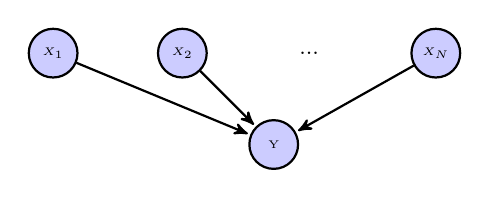
\begin{tikzpicture}[->,>=stealth',shorten >=1pt,auto,node distance=1cm,
  thick,main node/.style={observed}, hidden/.style={empty}]

 %nodes
\node[main node](1){$X_{1}$};
\node[main node, right=of 1](2){$X_{2}$};
\node[hidden, right=of 2](3){$...$};
\node[main node, right=of 3](4){$X_{N}$};
\node[main node, below right=of 2](5){Y};
 \path[every node/.style={font=\sffamily\small}]
    (1) edge (5)
    	(2) edge (5)
    (4) edge (5);
	
\end{tikzpicture}
\caption{Causal model for the parallel bandits problem.\label{fig:causalStructure}}
\end{figure}

In each round of the game, the learner either purely observes by selecting $do()$ or chooses a single variable to intervene on and the value to set it to. 
The remainder of the variables are simultaneously set by independently biased coin flips. 
The value of all variables are then used to determine the distribution of rewards for that round.
Formally, when not intervened upon we assume that each $X_i \sim \bernoulli(q_i)$ where $\vec{q} = (q_1, \ldots, q_N) \in [0,1]^N$ so that $q_i = \P{X_i = 1}$.
\todom{Should $Y$ be 0-1 valued or real everywhere?}
The value of the reward variable is distributed as $Y = r(\vec{X}) + \eta$ where $r : \{0,1\}^N \to \R$ is an arbitrary, fixed, and unknown function and $\eta$ is $1$-subgaussian noise with a distribution that may depend on $\vec{X}$.
In the farming example, this choice of $Y$ models the fixed, noisy but unknown dependence of crop yield on the temperature, soil, and moisture.

\todom{$i,j$ notation to $a \in \actions$}
In our analysis below, we will often use the pair $(i,j)$ for $i \in \{1, \ldots, N\}$ and $j \in \{0,1\}$ as a shorthand for the intervention $do(X_i = j)$.
We will also make use of the expansion of the expected reward for $do(X_i = j)$:
\eq{
\mu_{i,j} 
&= \E{r(X)|do(X_i = j)} \\
&= \sum_{\boldsymbol{x} \in \set{0,1}^N : x_i = j} r(\boldsymbol{x})  \prod_{k \neq i} q_k^{x_k} (1 - q_k)^{1-x_k}\,.  
}
The sum and product use the restrictions $x_i = j$ and $k \ne i$ because the intervention forces $X_i = j$ with probability 1.
The optimal intervention is denoted $(i^*,j^*) = \argmax_{i,j} \mu_{i,j}$ and the corresponding optimal reward is $\mu^* = \mu_{i^*,j^*}$. 
Note that the expected reward of the optimal intervention is at least as large as the expected reward for doing nothing.



\subsection{The Parallel Bandit Algorithm}
\label{sub:par-bandit-alg}

\begin{algorithm}[h]
\caption{Causal Best Arm Identification}\label{alg:simple}
\begin{algorithmic}[1]
\STATE {\bf Input:} Total rounds $T$, causal graph $\mathcal{G}$, allowable interventions $\actions$. 
\FOR{$t \in 1,\ldots,(T - 1) / 2$}
\STATE Perform empty intervention $do()$; observe $\vec{x}_t$ and $r_t$
\ENDFOR
\FOR{$a = do(X_i = x) \in \actions$}
\STATE Count times $X_i = x$ seen: $T_a = \sum_{t=1}^{T/2} \ind{x_{t,i} = x}$
\STATE Estimate reward: $\hat{\mu}_a = \frac{1}{T_a} \sum_{t=1}^{T/2} \ind{x_{t,i} = x} r_t$
\STATE Estimate probabilities: $\hat{p}_a = \frac{2 T_a}{T-1}$ and $\hat{V}_a = \frac{1}{\hat{p}_a}$
\ENDFOR
\STATE Compute $\hat{m} = m(\hat{\vec{V}})$ and $A = \set{a \in \actions \colon \hat{V}_a \geq \hat{m}}$.
\STATE Let $T_A := \frac{T-1}{2 |A|}$ be times to sample each $a\in A$.
\FOR{$a = do(X_i = x) \in A$}
\FOR{$t \in 1,\ldots,T_A$}
\STATE Intervene with $a$ and observe $r_t$
\ENDFOR
\STATE Re-estimate $\hat{\mu}_a = \frac{1}{T_A} \sum_{t=1}^{T_A} r_t$
\ENDFOR
\RETURN estimated optimal $\hat{a}^* \in \argmax_{a\in\actions} \hat{\mu}_a$
\end{algorithmic}
\end{algorithm}

\begin{theorem}\label{thm:uq-simple}
Algorithm \ref{alg:simple} satisfies
\eq{
\simpleregret \in \bigo{\sqrt{\frac{m}{T}\log\left(\frac{NT}{m}\right)}}\,.
}
\end{theorem}

Note that algorithms designed for finite-armed bandits would explore interventions more uniformly and achieve a regret of $\Omega(\sqrt{N/T})$.
Since $m$ is typically much smaller than $N$ we anticipate that the new algorithm will significantly outperform classical bandit algorithms in
this setting.
We prove a lower bound on the simple regret that matches up to logarithmic factors the upper bound given in Theorem \ref{thm:uq-simple}

\begin{theorem}\label{thm:lower}
Suppose $\boldsymbol{q}$ satisfies $m(\boldsymbol{q}) = m$.
Then for all strategies there exists a reward function such that
\eq{
\simpleregret \geq \frac{\frac{m}{2e} - 1}{m} \sqrt{\frac{2m}{3T}} = \Omega\left(\sqrt{\frac{m}{T}}\right)\,.
}
\end{theorem}

\ifsup
The proof of Theorems \ref{thm:uq-simple} and \ref{thm:lower} may be found in Sections \ref{sec:thm:uq-simple} and \ref{sec:thm:lower}.
\else
The proof of Theorems \ref{thm:uq-simple} and \ref{thm:lower} may be found in the supplementary material.
\fi






%%%%%%%%%%%%%%%%%%%%%%%%%%%%%%%%%%%%%%%%%%%%%%%%%
% UPPER BOUND ON SIMPLE REGRET GENERAL CASE
%%%%%%%%%%%%%%%%%%%%%%%%%%%%%%%%%%%%%%%%%%%%%%%%%
\section{Regret Bounds for General Graphs}
\label{sec:simple-regret-general}

\newcommand{\calP}{\mathcal P}
\newcommand{\calA}{\mathcal A}
\newcommand{\x}{\boldsymbol{x}}

We now consider the more general problem where the graph structure is known, but arbitrary.
As before $Y$ is the target variable and $\P{Y=1|X} = r(X)$ is the expected reward given $X$.
We let $\calP_i \subseteq \set{1,\ldots,N}$ denote the parents of variable $X_i$ so the joint distribution over $X$ may be written as
\eq{
\P{X = x} = \prod_{i=1}^N \P{X_i = x_i|X_j = x_j \text{ for all } j \in \calP_i}\,.
}
Throughout this section we assume that the causal structure and conditional distributions of $X$ are known,
which allows us to compute the above quantity for arbitrary $x \in \Omega = \set{0,1}^N$. Given the learner intervens by $do(X_i = j)$
leads to
\eq{
&\Pn{ij}{X = x} = \P{X = x|do(X_i = j)} \\
&\qquad =\prod_{k \neq i} \P{X_k = x_k|X_j = x_j \text{ for all } j \in \calP_k}\,.
}
The expected reward by making the intervention $do(X_i = j)$ is
\eq{
\mu_{ij} = \sum_{x \in \Omega} \P{X = x|do(X_i = j)} r(x)\,.
}
The problem of learning the optimal intervention is made more complicated than the simple case because of 
the dependencies between the random variables. Learning from observational data is no longer straightforward
because variables can be correlated through their parents. Consider, for example, the causual graph below where $X_1$
deterministically causes $X_2$ and $X_3$, which ensures that $X_2 = X_3$ for all observational data. Now suppose $r(X) = \ind{X_2 \neq X_3}$,
then intervening on either $X_2$ or $X_3$ is optimal. But the positive reward is never observed from observational samples, despite
the fact that $\P{X_2 = 1} = \P{X_3 = 1} = \frac{1}{2}$.
\begin{figure}[h]
\centering
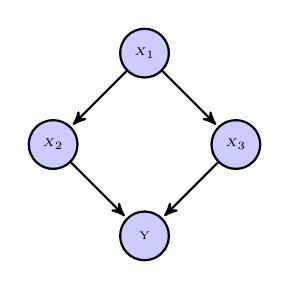
\begin{tikzpicture}[->,>=stealth',shorten >=1pt,auto,node distance=1cm,
  thick,main node/.style={observed}, hidden/.style={empty}]
\node[main node](1){$X_1$};
\node[main node, below left=of 1](2){$X_2$};
\node[main node, below right=of 1](3){$X_3$};
\node[main node, below right=of 2](4){Y};
 \path[every node/.style={font=\sffamily\small}]
    (1) edge (2)
    (1) edge (3)
    (3) edge (4)
    (2) edge (4);
\end{tikzpicture}
\eq{
\P{X_1 = 1} &= \frac{1}{2} \\
\P{X_2 = j|X_1 = j} &= 
\P{X_3 = j|X_1 = j} = 1\,.
}
\caption{}\label{fig:causalStructure_confounded}
\end{figure} 

Another difficulty is that it is no longer sufficient to learn about $\mu_{ij}$ exclusivly from observational data and when $do(X_i = j)$ is chosen.
We can also learn about the reward for intervening on one variable from rounds in which we actually set a different variable.
Consider the graph in Figure \ref{fig:causalchain}, where each variable deterministically takes the value of its parent, $X_k = X_{k-1}$ 
for $k\in {2,\ldots,N}$ and $\P{X_1} = 0$. 
We can learn the reward for all the interventions $do(X_i = 1)$ simultaneously by selecting $do(X_1 = 1)$. 

\begin{figure}[h]
\centering
\caption{A causal chain graph}.
\label{fig:causalchain}
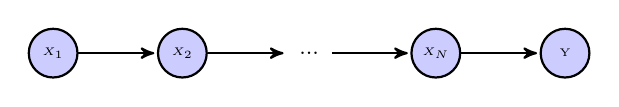
\begin{tikzpicture}[->,>=stealth',shorten >=1pt,auto,node distance=1cm,
  thick,main node/.style={observed}, hidden/.style={empty}]
\node[main node](1){$X_{1}$};
\node[main node, right=of 1](2){$X_{2}$};
\node[hidden, right=of 2](3){$...$};
\node[main node, right=of 3](4){$X_{N}$};
\node[main node, right=of 4](5){Y};
 \path[every node/.style={font=\sffamily\small}]
    (1) edge (2)
  	(2) edge (3)
    (3) edge (4)
    (4) edge (5);
\end{tikzpicture}
\end{figure} 



Before the algorithm we introduce the truncated importance weighted estimator, which we will use to learn about the returns of 
specific interventions from observational data, or by intervening on other variables. Let $P$ and $Q$ be distributions on $\Omega$.
We would like to estimate
\eq{
\mu_Q = \EE_Q r(x) = \sum_{x \in \Omega} Q(x) r(x) 
}
using samples $X \in \Omega$ and $Y \in \set{0,1}$ where $X \sim P$ and $Y = 1$ with probability $r(X)$. Ultimately we will be interested
in the case that 
$Q(x) = P(x|do(X_i = j))$
and where $P(x) = P(x|do())$ or $P(x|do(X_k = l))$, but for now we keep things general.
Define random variable $R(x) = Q(x)/P(x)$ and estimator $Z$ by
\eqn{
\label{eq:truncated}
Z = Y R \ind{R < B}\,,
}
which trivially satisfies $|Z| \leq B$ surely.
Note that the usual importance weighted estimator would be $YR$, which if $Q$ is absolutely continuous with respect to $P$ satisfies $\EE_P YR = \mu$. Unfortunately
this estimator may suffer from poor concentration, a problem that can be mitigated via the truncation in (\ref{eq:truncated}) at the cost of some bias.
Computing the expectation we see
\eq{
\EE_P[Z] = \mu - \beta\,.
}
where $\beta \geq 0$ is the negative bias and satisfies
\eq{
\beta \leq \Q{R \geq B}\,.
}
Bounding the variance is also straightforward.
\eq{
\Var[Z] 
&\leq \EE[Z^2] 
=\sum_x \P{X = x} Z(x)^2 \\
&\leq \sum_x \P{X = x} \left(\frac{\Q{X = x}}{\P{X = x}}\right)^2 \\
&= \sum_x \Q{X = x} \frac{\Q{X = x}}{\P{X = x}} 
= V\,.
}
The bias can be controlled in terms of $V$ via Markov's inequality.
\eq{
\beta 
\leq \Q{R \geq B} 
\leq \frac{\EE_Q[R]}{B}
= \frac{V}{B}\,.
}
The point is that $B$ can be tuned to trade the bias against the concentration of the estimator,
the latter of which will be controlled via Bernstein's inequality. 

Let $\operatorname P_{ij}$ be the measure on $\Omega$ with $\Pij{X = x} = \P{X = x|do(X_i = j)}$.
As in the previous section, the algorithm for learning an optimal intervention on a general graph will 
collect $T/2$ observational samples by choosing $do()$. It then chooses $do(X_i = j)$ 
exactly $N_{ij}$ times, where $N_{ij}$ will be chosen shortly. For each $i$ it computes an estimate $\hat \mu_{ij}$ of $\mu_{ij}$ via
a mixture of truncated importance weighted estimators.
\eq{
\hat \mu_{ij} 
= 
\frac{
  \eta_{ij} \sum_{t=1}^{T/2} \frac{Z_{ij}(t)}{T/2} + \sum_{kl \in \calA_{ij}} \eta_{ijkl} \sum_{t=1}^{N_{kl}} \frac{Z_{ijkl}(t)}{N_{kl}}}
    {\eta_{ij} + \sum_{kl \in \calA_{ij}} \eta_{ijkl}}\,,
}
where 
\eq{
\calA_{ij} = \set{ij} \cup \set{kl : k \text{ is an ancestor of } i \text{ and } l \in \set{0,1}}
}
and
\eq{
\eta_{ij} &= \frac{T/2}{V_{ij}} &
V_{ij} &= \EE_{\operatorname{P}_{ij}} \left[\frac{\Pn{ij}{X = x}}{\P{X = x}}\right] \\
\eta_{ijkl} &= \frac{N_{kl}}{V_{ijkl}} &
V_{ijkl} &= \EE_{\operatorname{P}_{ij}} \left[\frac{\Pn{ij}{X = x}}{\Pn{kl}{X = x}}\right]
}

The following theorem controls the concentration of $\hat \mu_{ij}$ about $\mu_{ij}$. 
\ifsup
The proof may be found in Appendix \ref{sec:thm:estimate}.
\else
The proof follows from an application of Bernstein's inequality and may be found in the supplementary material.
\fi

\begin{theorem}\label{thm:estimate}
The estimator $\hat \mu_{ij}$ satisfies:
\eq{
\P{\left|\hat \mu_{ij} - \mu\right| \geq \sqrt{\frac{1}{\sum_{kl \in \calA_{ij}} \frac{N_{kl}}{V_{ijkl}}} \log\frac{1}{\delta}}} \leq \delta\,.
}
\end{theorem}


All that remains is to choose $N_{ij}$ to minimise the worst-case approximation error in the bound above over all $i$ and $j$.
This is acheived by finding the smallest $\epsilon > 0$ such that {\sc CheckValid} returns true (see Algorithm \ref{alg:alloc}).

\todot{Topological sort}
\begin{algorithm}[H]
\caption{CheckValid}\label{alg:alloc}
\begin{algorithmic}
\STATE {\bf Input:} $\epsilon > 0$, $\delta > 0$, $\operatorname P_{ij}$ for all $ij$
\STATE Compute $o_1,\ldots,o_N \in \set{1,\ldots,N}$
\FOR{$i \in \set{o_1,\ldots,o_N}$ and $j \in \set{0,1}$}
\STATE Compute variances:
\eq{
\forall k \in \calA_i,\, l \in \set{0,1} \quad
V_{ijkl} = \frac{1}{N_{kl}} \EE_{\operatorname P_{ij}}\!\! \left[\frac{\Pij{x}}{\Pkl{x}}\right] 
}
\STATE Compute variance for learning from observational data:
\eq{
V_{ij} = \frac{2}{T} \EE_{\operatorname P_{ij}} \!\!\left[\frac{\Pij{x}}{\P{x}}\right]
}
\STATE Compute required budget: 
\eq{
N_{ij} = \max\set{0, \ceil{\frac{1}{\epsilon^2} - \sum_{k \in \calA_i} \sum_{l \in \set{0,1}} \frac{1}{V_{ijkl}} - \frac{1}{V_{ij}}}}\,.
} 
\ENDFOR
\STATE {\bf if $\sum_{ij} N_{ij} \leq T/2$} {\bf return} true {\bf else return} false
\end{algorithmic}
\end{algorithm}

\todot{discuss role of $delta = 1/(NT)$}
\todot{define $Z_{ijkl}(t)$ etc.}
\todot{Define $B_{ijkl}$}
\begin{theorem}
Let $\epsilon > 0$ be the smallest value of $\epsilon$ such that Algorithm \ref{alg:alloc} returns true and let $IJ = \argmax_{ij} \hat \mu_{ij}$.
Then $\mu^* - \E \mu_{IJ} \leq \epsilon + 1/T$.
\end{theorem}


\subsection*{Comparison to Simple Setting}

In Section \ref{sec:simple-regret} we assumed a simple graph structure and unknown distributions on $X_i$, which were then learned from observational
data. In contrast, in this section we have allow arbitrary (known) graphs, but assumed the distribution on $X$ was known. 
Using the approach in this section on the simple graph with known distribution leads to 
\eq{
\EE \mu^* - \EE \mu_{IJ} \in \bigo{\sqrt{\frac{m}{T} \log \frac{N}{\delta}}}\,, 
}
which is the same bound as in the previous section. 
\todot{finish this}






 

%%%%%%%%%%%%%%%%%%%%%%%%%%%%%%%%%%%%%%%%%%%%%%%%%
% EXPERIMENTS
%%%%%%%%%%%%%%%%%%%%%%%%%%%%%%%%%%%%%%%%%%%%%%%%%
\section{Experiments}
\label{sec:experiments}

\documentclass{article}
\usepackage{tikz} 
\usepackage[utf8]{inputenc}
\usepackage{amsmath}
\usepackage{listings}
\usepackage{amsfonts}
\usepackage{amssymb}
\usepackage{tabularx}
\usepackage{enumitem}
\usepackage{algorithm}% http://ctan.org/pkg/algorithm
\usepackage[noend]{algpseudocode}% http://ctan.org/pkg/algorithmicx
\usepackage{tikz}
\usepackage{graphicx}


\usepackage{subcaption}
\usepackage{multicol,caption}
\usepackage{geometry}
 \geometry{
 a4paper,
 total={210mm,297mm},
 left=20mm,
 right=20mm,
 top=20mm,
 bottom=20mm,
 }

\usetikzlibrary{arrows,positioning,shapes,fit} 
\pgfarrowsdeclarecombine{ring}{ring}{}{}{o}{o}
\thispagestyle{empty}
\DeclareMathOperator{\ringarrow}{\raisebox{0.5ex}{\tikz[baseline]{\draw[ring->](0,0)--(2em,0);}}}

\definecolor{talk}{HTML}{729FCF}
\definecolor{talk2}{HTML}{E8A753}
\definecolor{grey}{HTML}{DBDCDD}
\renewcommand{\vec}[1]{\boldsymbol{#1}}
\tikzset{
    %Define standard arrow tip
    >=stealth',
    %Define style for boxes
    observed/.style={
   	circle,
   	rounded corners,
   	draw=black, thick,
   	minimum width=2.3em,
   	minimum height=2.3em,
   	font=\footnotesize,
   	text centered,
   	fill=talk!50
   },
   latent/.style={
   	circle,
   	rounded corners,
   	draw=black, thick, dashed,
   	minimum width=2.2em,
   	minimum height=2.2em,
   	font=\footnotesize,
   	text centered
   },
    % Define arrow style
    pil/.style={
           o->,
           thick,
           shorten <=2pt,
           shorten >=2pt,},
    sh/.style={ shade, shading=axis, left color=red, right color=green,
    shading angle=45 },
observedrect/.style={
	rectangle,
	rounded corners,
	draw=black, thick,
	minimum width=3em,
	minimum height=1.5em,
	font=\footnotesize,
	text centered,
	fill=talk2!80
},  
 target/.style={
	circle,
	rounded corners,
	draw=black, thick,
	minimum width=2.3em,
	minimum height=2.3em,
	font=\footnotesize,
	text centered,
	fill=talk2!80
},
empty/.style={
	circle,
	rounded corners,
	minimum width=.5em,
	minimum height=.5em,
	font=\footnotesize,
	text centered,
},
}
   
\begin{document}
%\pagestyle{empty}

 \begin{figure}[ht]
 	\begin{subfigure}[t]{0.49\textwidth}
 		\centering    
 		\includegraphics[width=\textwidth]{experiment1_20161020_1247.pdf}
 		\caption{Simple regret vs $m(\boldsymbol{q})$ for fixed horizon $T=400$ and number of variables $N = 50$}
 		\label{fig:simple_vs_m}
 	\end{subfigure}\hfill
 	\begin{subfigure}[t]{0.49\textwidth}
 		\centering
 		\includegraphics[width=\textwidth]{experiment3_20161020_1252.pdf}
 		\caption{Simple regret vs horizon, $T$, with $N = 50$, $m=2$ and fixed $\epsilon = .3$}
 		\label{fig:simple_vs_T}
 	\end{subfigure}
 \end{figure}

\end{document}


%%%%%%%%%%%%%%%%%%%%%%%%%%%%%%%%%%%%%%%%%%%%%%%%%
% DISCUSSION
%%%%%%%%%%%%%%%%%%%%%%%%%%%%%%%%%%%%%%%%%%%%%%%%%
\section{Discussion \& Future Work}
\label{sec:discussion}

Algorithm~\ref{alg:general} for general causal bandit problems adaptively estimates the reward for all allowable interventions $a \in \calA$ over $T$ rounds by sampling and applying interventions from a distribution $\eta$.
Theorem~\ref{thm:general} shows that this algorithm has (up to log factors) simple regret that is $\bigo{\sqrt{m(\eta)/T}}$ and that the parameter $m(\eta)$ is always less than $N$.
The value of $m(\eta)$ is a uniform bound on the variance of the reward estimators $\hat{\mu}_a$ and, intuitively, problems where all variables' values in the causal model ``occur naturally'' when interventions are sampled from $\eta$ will have low values of $m(\eta)$.

The main practical drawback of Algorithm~\ref{alg:general} is that both the estimator terms $Z_a$ and the optimal sampling distribution $\eta^*$ (\ie, the one that minimises $m(\eta)$) require knowledge of the conditional distributions $P_a$ for all $a \in \calA$.
In contrast, in the special case of parallel bandits, Algorithm~\ref{alg:simple} uses the $do()$ action to effectively estimate $m(\eta)$ and the rewards then re-samples the interventions with variances that are not bound by $\hat{m}(\eta)$.
Despite these extra estimates, Theorem~\ref{thm:lower} shows that this approach is optimal (up to log factors).
Finding an algorithm that only requires the causal graph and lower bounds for its simple regret in the general case is left as future work.

\paragraph{Making Better Use of the Reward Signal}
Existing algorithms for best arm identification are based on ``successive rejection'' (SR) of arms based on UCB-like bounds on their rewards~\citep{Even-Dar2002}.
In contrast, our algorithms completely ignore the reward signal when developing their arm sampling policies and only use the rewards when estimating $\hat{\mu}_a$.
Incorporating the reward signal into our sampling techniques or designing more adaptive reward estimators that focus on high reward interventions is an obvious next step.
This would likely improve the poor performance of our causal algorithm relative to the sucessive rejects algorithm for large $m$, as seen in Figure~\ref{fig:simple_vs_m}.
For the parallel bandit the required modifications should be quite straightforward. The idea would be to adapt the algorithm to essentially use successive elimination in
the second phase so arms are eliminated as soon as they are provably no longer optimal with high probability. In the general case a similar modification is also possible
by dividing the budget $T$ into phases and optimising the sampling distribution $\eta$, eliminating arms when their confidence intervals are no longer overlapping. Note
that these modifications will not improve the minimax regret, which at least for the parallel bandit is already optimal. For this reason we prefer to emphasize 
the main point that causal structure should be exploited when available. Another observation is that Algorithm \ref{alg:general} is actually using a fixed design, which
in some cases may be preferred to a sequential design for logistical reasons. This is not possible for Algorithm \ref{alg:simple}, since the $\vec{q}$ vector is unknown.

\paragraph{Cumulative Regret}
Although we have focused on simple regret in our analysis, it would also be natural to consider the cumulative regret.
In the case of the parallel bandit problem we can slightly modify the analysis from \citep{wu2015online} on bandits with side information 
to get near-optimal cumulative regret guarantees. They consider a finite-armed bandit model with side information where in reach round
the learner chooses an action and receives a Gaussian reward signal for all actions, but with a known variance that depends on the chosen action.
In this way the learner can gain information about actions it does not take with varying levels of accuracy. The reduction follows by substituting
the importance weighted estimators in place of the Gaussian reward. In the case that $\vec{q}$ is known this would lead to a known variance
and the only (insignificant) difference is the Bernoulli noise model. In the parallel bandit case we believe this would lead to near-optimal cumulative regret,
at least asymptotically. 

%Their model assumes the rewards for all arms $a$ are Gaussian with mean $\mu_a$ and variance $\sigma^2_{ab}$ and that playing an arm $a$ will reveal a side observation $Y_{ab}$ of the reward for all arms $b$ distributed with mean $\mu_b$ and variance $\sigma^2_{ab}$.
%We can build a similar dependence structure with variances for a Bernoulli reward variable that is derived from the $\vec{q}$ vector of probabilities.
%\todom{Check this!}
%Even though the original results are for Gaussian rewards we believe the analysis will go through largely unchanged.

The parallel bandit problem can also be viewed as an instance of a time varying graph feedback problem \citep{Alon2015,Kocak2014}, where at each timestep the feedback graph $G_t$ is selected stochastically, dependent on $\boldsymbol{q}$, and revealed after an action has been chosen. The feedback graph is distinct from the causal graph. A link $A \rightarrow B$ in $G_t$ indicates that selecting the action $A$ reveals the reward for action $B$. For this parallel bandit problem, $G_t$ will always be a star graph with the action $do()$ connected to half the remaining actions. However, \citet{Alon2015,Kocak2014} give adversarial algorithms, which when applied to the parallel bandit problem obtain the standard bandit regret. A malicious adversary can select the same graph each time, such that the rewards for half the arms are never revealed by the informative action. This is equivalent to a nominally stochastic selection of feedback graph where $\boldsymbol{q} = \boldsymbol{0}$. 

% \cite{Lelarge2012} consider a stochastic version of the graph feedback problem, but with a fixed graph available to the algorithm before it must select an action. In addition, their algorithm is not optimal for all graph structures and fails, in particular, to provide improvements for star like graphs as in our case. \cite{Buccapatnam2014} improve the dependence of the algorithm on the graph structure but still assume the graph is fixed and available to the algorithm before the action is selected. 


\paragraph{Causal Models with Non-Observable Variables}
If we assume knowledge of the conditional \textit{interventional} distributions $P_a$ our analysis applies unchanged to the case of causal models with 
non-observable variables. For example, if we had access to a data set of \textit{experiments} in which the reward variable $Y$ was not 
available from which to build estimates of $P_a$. Some of the interventional distributions $P_a$ may be non-identifiable meaning we can not obtain prior estimates for $P_a$ from 
even an infinite amount of observational data. Even if all variables are observable and the graph is known, if the conditional distributions are unknown, then Algorithm
\ref{alg:general} cannot be used. Estimating these quantities while simultaneously minimising the simple regret is an interesting and challenging open problem.


% In this case, some conditional distributions may be non-identifiable. 
% The corresponding actions can be immediately added to the set $A$ prior to collecting any data. 
% We can then use the same algorithm as in the case where there are no latent variables, except that we will have to use the more general do-calculus rather than simply adjusting for the parents to write the expression for each action in terms of observational data.
% Combining our estimation techniques with insights from \citet{Bareinboim2015} for handling unobserved confounders would be worth investigation.


% More generally, assuming causal structure creates more complex types of side information, such as that shown in equation \ref{eq:estimation_transfer}. In this case, selecting one action does not fully reveal an alternate action but provides some information towards an estimate. The quality of the estimate notably depends not only on the number of times that action was selected. For example, to get a good estimate for $X_1 = 1$ by intervening on $X_2$ requires us to sample both $X_2=0$ and $X_2=1$, in proportions dependent on $q_2$. This more complex side information does not fit within the graph feedback framework.


\paragraph{Partially or Completely Unknown Causal Graph}
A much more difficult generalisation would be to consider causal bandit problems where the causal graph is completely unknown or known to be a member of class of models.
The latter case arises naturally if we assume free access to a large observational dataset, from which the Markov equivalence class can be found via causal discovery techniques. 
Work on the problem of selecting experiments to discover the correct causal graph from within a Markov equivalence class~\cite{Eberhardt2005,eberhardt2010causal,hauser2014two,Hu2014b} could potentially be incorporated into a causal bandit algorithm.
In particular, \citet{Hu2014b} show that only $\bigo{\log \log n}$ multi-variable interventions are required on average to recover a causal graph over $n$ variables once purely observational data is used to recover the ``essential graph''.
Simultaneously learning a completely unknown causal model while estimating the rewards of interventions without a large observational dataset would be much more challenging.

% (Partially known structure)
% Key results $bigo(n)$ singleton or $bigo(log log n)$ multi-variate experiments are required.
% - Focus on minimizing the number of experiments that must be performed. Examples of active versus online learning. The cost of experiments constant or at least known. 

% (Unknown Structure)
% If we need to learn the structure, in an online environment. 
% Experiment is much, much more revealing than inference from observational data. We would expect it to dominate. 



%\pagebreak
{\small\bibliography{libraryicml}}
\bibliographystyle{apalike}

\ifsup


%%%%%%%%%%%%%%%%%%%%%%%%%%%%%%%%%%%%%%%%%%%%
% PROOF OF SIMPLE REGRET UPPER BOUND
%%%%%%%%%%%%%%%%%%%%%%%%%%%%%%%%%%%%%%%%%%%%
\section{Proof of Theorem \ref{thm:uq-simple}}\label{sec:thm:uq-simple}

Assume without loss of generality that $q_1 \leq q_2 \leq \ldots \leq q_N \leq 1/2$. The assumption is non-restrictive since all variables
are independent and permutations of the variables can be pushed to the reward function.
The proof of Theorem \ref{thm:uq-simple} requires some lemmas, the first of which is an immediate consequence of the Chernoff bound.


\begin{lemma}\label{lem:conc1}
Let $i \in \set{1,\ldots, N}$ and $\delta > 0$. Then
\eq{
\P{\left|\hat q_i - q_i\right| \geq \sqrt{\frac{6q_i}{T} \log \frac{2}{\delta}}} \leq \delta\,.
}
\end{lemma}

\begin{lemma}\label{lem:conc2}
Let $X_1,X_2\ldots,$ be a sequence of random variables with $X_i \in [0,1]$ and $\EE X_i = p$ and $\delta \in [0,1]$.
Then 
\eq{
\P{\exists t \geq n_0 : \left|\frac{1}{t} \sum_{s=1}^t X_s - p\right| \geq \sqrt{\frac{2}{n_0} \log \frac{2}{\delta}}} \leq 4\delta\,.
}
\end{lemma}

\begin{proof}
For $\delta \geq 1/4$ the result is trivial. Otherwise 
by Hoeffding's bound and the union bound:
\eq{
\P{\exists t \geq n_0 : \left|\frac{1}{t} \sum_{s=1}^t X_s - p\right| \geq \sqrt{\frac{2}{n_0} \log \frac{2}{\delta}}} 
&\leq \sum_{t = n_0}^\infty \P{\left|\frac{1}{t} \sum_{s=1}^t X_s - p\right| \geq \sqrt{\frac{2}{n_0} \log \frac{2}{\delta}}} \\
&\leq 2\sum_{t=n_0}^\infty \exp\left(-\frac{t}{n_0} \log \frac{2}{\delta}\right) 
\leq 4\delta\,. \qedhere
}
\end{proof}



\begin{lemma}\label{lem:m_est}
Let $\delta \in (0,1)$ and assume $T \geq 48m \log\frac{2N}{\delta}$. Then
\eq{
\P{2m(\vec{q}) / 3 \leq m(\vec{\hat q}) \leq 2m(\vec{q})} \geq 1 - \delta\,.
}
\end{lemma}

\begin{proof}
Let $F$ be the event that there exists and $1 \leq i \leq N$ for which
\eq{
\left|\hat q_i - q_i\right| \geq \sqrt{\frac{6q_i}{T} \log \frac{2N}{\delta}}\,.
}
Then by the union bound and Lemma \ref{lem:conc1} we have $\P{F} \leq \delta$. The result will be completed by showing that
when $F$ does not hold we have $2m(\vec{q})/3 \leq m(\vec{\hat q}) \leq 2m(\vec{q})$.
Towards this end recall that $m(\vec{q}) = \min\set{i : q_i \geq 1 / i}$.
Therefore for $i > m$ we have $q_i \geq q_m \geq 1/m$ and so by Lemma \ref{lem:conc1} we have
\eq{
\frac{3}{4} 
&\geq \frac{1}{2} + \sqrt{\frac{3}{T} \log \frac{2N}{\delta}} 
\geq q_i + \sqrt{\frac{6q_i}{T} \log \frac{2N}{\delta}} 
\geq \hat q_i \\
&\geq q_i - \sqrt{\frac{6q_i}{T} \log \frac{2N}{\delta}}
\geq q_i - \sqrt{\frac{q_i}{8m}}
\geq \frac{1}{2m}\,.
}
Therefore by the pigeonhole principle we have $m(\vec{\hat q}) \leq 2m$.
For the other direction we proceed in a similar fashion. Since the failure event $F$ does not hold we have for $i \leq m$ that
\eq{
\hat q_i 
\leq q_i + \sqrt{\frac{6q_i}{T} \log\frac{2N}{\delta}} 
\leq \frac{1}{m} \left(1 + \sqrt{\frac{1}{8}}\right)
\leq \frac{3}{2m}\,.
}
Therefore $m(\vec{\hat q}) \geq 2m(\vec{q}) / 3$ as required. 
\end{proof}

\begin{proof}[Proof of Theorem \ref{thm:uq-simple}]
Let $\delta = m = m(\vec{q}) / N$. Then by Lemma \ref{lem:m_est} we have 
\eq{
\P{2m/3 \leq m(\vec{\hat q}) \leq 2m} \geq 1 - \delta\,.
}
Recall that $A = \set{a \in \actions : \hat p_a \leq 1/m(\vec{\hat q})}$. Then
for $a \in A$ the algorithm estimates $\mu_a$ from $T/(2m(\vec{\hat q})) \geq T/(4m)$ samples.
Therefore by Hoeffding's inequality and the union bound we have
\eq{
\P{\exists a \in A : |\mu_a - \hat \mu_a| \geq \sqrt{\frac{8m}{T} \log\frac{2N}{\delta}}} \leq \delta\,.
}
For arms not in $a$ we have $\hat p_a \geq 1/m(\vec{\hat q}) \geq 1/(2m)$.
Therefore if $a = do(X_i = j)$, then 
\eq{
\hat p_a = \frac{2}{T} \sum_{t=1}^{T/2} \ind{X_i = j} \geq \frac{1}{2m}\,. 
}
Therefore $\sum_{t=1}^{T/2} \ind{X_{t,i} = j} \geq T/4m$
and by Lemma \ref{lem:conc2} we have
\eq{
\P{\sum_{t=1}^{T/2} \ind{X_i = j} \geq \frac{T}{4m} \text{ and } \left|\hat \mu_a - \mu_a\right| \geq \sqrt{\frac{8m}{T} \log \frac{2N}{\delta}}} \leq 4\delta / N\,.
}
Therefore with probability at least $1 - 6\delta$ we have
\eq{
(\forall a \in \actions) \qquad |\hat \mu_a - \mu_a| \leq \sqrt{\frac{8m}{T} \log \frac{N}{\delta}} = \epsilon\,.
}
If this occurs, then 
\eq{
\mu_{\hat a^*} \geq \hat \mu_{\hat a^*} - \epsilon \geq \hat \mu_{a^*} - \epsilon \geq \mu_{a^*} - 2\epsilon\,.
}
Therefore
\eq{
\mu^* - \EE[\mu_{\hat a^*}] 
\leq 6\delta + \epsilon 
\leq \frac{6m}{T} + \sqrt{\frac{32m}{T} \log \frac{NT}{m}}\,, 
}
which completes the result.
\end{proof}

%%%%%%%%%%%%%%%%%%%%%%%%%%%%%%%%%%%%%%%%%%%%
% LOWER BOUND
%%%%%%%%%%%%%%%%%%%%%%%%%%%%%%%%%%%%%%%%%%%%
\section{Proof of Theorem \ref{thm:lower}}\label{sec:thm:lower}

Assume without loss of generality that $q_1 \leq q_2 \leq \ldots \leq q_N \leq 1/2$.
For each $i$ define reward function $r_i$ by
\eq{
r_0(\boldsymbol{X}) &= \frac{1}{2} &
r_i(\boldsymbol{X}) &= \begin{cases}
\frac{1}{2} + \epsilon & \text{if } X_i = 1 \\
\frac{1}{2} & \text{otherwise}\,,
\end{cases}
}
where $1/4 \geq \epsilon > 0$ is some constant to be chosen later.
We abbreviate $R_{T,i}$ to be the expected simple regret incurred when interacting with the
environment determined by $\boldsymbol{q}$ and $r_i$. Let $P_i$ be the corresponding measure
on all observations over all $T$ rounds and $\EE_i$ the expectation with respect to $P_i$. By Lemma 2.6 by \cite{Tsy08} we have
\eq{
\Prz{I_T = i} + \Pri{I_T \neq i} \geq \exp\left(-\KL(P_0, P_i)\right)\,,
}
where $\KL(P_0, P_i)$ is the KL divergence between measures $P_0$ and $P_i$.
Let $T_i(T) = \sum_{t=1}^T \ind{a_t = do(X_i = 1)}$ be the total number of times the learner intervenes on variable $i$ by setting it to $1$.
Then for $i \leq m$ we have $q_i \leq 1/m$ and the KL divergence between $P_0$ and $P_i$ may be bounded using the telescoping property (chain rule) and
by bounding the local KL divergence by the $\chi$-squared distance as by \cite{Auer1995}. This leads to 
\eq{
\KL(P_0, P_i) 
&\leq 6\epsilon^2 \EE_0\left[\sum_{t=1}^T \ind{X_{t,i} = 1}\right] 
\leq 6\epsilon^2 \left(\EE_0 T_i(T) + q_i T\right) 
\leq 6\epsilon^2 \left(\EE_0 T_i(T) + \frac{T}{m}\right)\,.
}
Define set $A$ by $A = \set{i \leq m : \EE_0 T_i(T) \leq 2T / m}$.
Then for $i \in A$ and choosing $\epsilon = \sqrt{m/(18T)}$ we have
\eq{
\KL(P_0, P_i) \leq \frac{18T\epsilon^2}{m} = 1\,. 
}
Now $\sum_{i=1}^m \EE_0 T_i(T) \leq T$, which implies that $|A| \geq m/2$.
Therefore
\eq{
\sum_{i \in A} \Pri{I_T \neq i} 
&\geq \sum_{i \in A} \exp\left(-\KL(P_0, P_i)\right) - 1\\
&\geq \frac{|A|}{e} - 1 
\geq \frac{m}{2e} - 1\,.
}
Therefore there exists an $i \in A$ such that
\eq{
\Pri{I_T \neq i} \geq \frac{\frac{m}{2e} - 1}{m}\,.
}
Therefore
\eq{
R_{T,i} \geq \frac{1}{2} P_i(I_T \neq i) \epsilon \geq \frac{\frac{m}{2e} - 1}{2m} \sqrt{\frac{2m}{3T}}
}
as required.











\fi

\end{document}
